\documentclass{scrartcl}

\usepackage[ngerman]{babel}

\usepackage[utf8]{inputenc}
\usepackage{hyperref,xcolor,microtype,ifthen}
\usepackage{csquotes}
\usepackage{parskip}

\usepackage{graphicx}
\usepackage{svg}

\usepackage{helvet}
\renewcommand{\familydefault}{\sfdefault}
\fontfamily{phv}\selectfont

\linespread{1.25}

\title{Mobile Application Development}
\subtitle{Eventure Dokumentation}
\date{\today}
\author{Alexander Rasputin, Maximilian Karthan, Jona Ruof}

\begin{document}

\maketitle
\newpage
\tableofcontents

\newpage

\section{Einleitung}
\subsection{Motivation}

Um die Kenntnisse im Bereich der mobile Anwendungsentwicklung zu vertiefen,
sollte im zweiten Teil des Mobile Application Projects eine eigene Applikation
entwickelt werden. Die Anwendung sollte dabei eine Problemstellung aus einem
frei wählbaren Themengebiet lösen. Die hier entwickelte \emph{Eventure} App
vereint viele verschieden Aspekte der mobile Anwendungsentwicklung und stellt
somit eine ausreichend komplexe Aufgabe dar.

Prägend für das Design von \emph{Eventure} ist der Begriff des \emph{Events}.
Als Event wird hier jede Art des lokalen, zeitlich begrenzten, sozialen
Ereignisses verstanden. So werden z.B. eine Theatervorstellung, ein
Volleyballspiel im Park oder eine Geburtstagsfeier als Events bezeichnet. Events
bieten Möglichkeiten zur sozialen Interaktion mit Freunden und Fremden und sind
damit relevant für das Leben aller Menschen. Gerade für ortsfremde Personen ist
es oftmal kompliziert an die relevanten Eckdaten (Zeit, Ort, etc. ...) eines
Events zu kommen. Da keine zentralisierte Sammelstelle für solche Information
existiert, sind diese meist in verschiedensten Medien zu finden oder werden nur
von Person zu Person weitergegeben. Daher scheint die Notwendigkeit einer
Applikation für das Entdecken von Events gegeben.

Es existieren bereits einige solcher Apps, welche allerdings (subjektiv
betrachtet) nicht einfach und intuitiv genug bedient werden können. So sind
insbesondere die Abläufe für das Finden und Erstellen von Events zu kompliziert
gestaltet. Zahlreiche Einstellungs- und Suchoptionen verschlechtern die
Bedienbarkeit zusätzlich.

\subsection{Ziel}

Das Ziel des Mobile Application Developments ist die Entwicklung einer Android
Applikation die das Entdecken und Erstellen von Events ermöglicht. Dabei sollte
die App besonders einfach zu bedienen sein. Die Probleme der bereits bekannten
Event Apps sollten gelöst oder zumindest entscheidend verbessert werden.
Außerdem sollen die Kenntnisse in der Android Programmierung weiter vertieft
werden, so dass am Ende des Projekts alle grundlegenden und einige
weiterführende Konzepte der mobilen Anwendungentwicklung bekannt sind.

\subsection{Aufbau}

In der folgenden Dokumentation werden in der Anforderungsanalyse zunächst die
funktionalen und nicht funktionalen Anforderungen der Applikation präsentiert.
Ebenfalls werden verwendeten Frameworks und die Architektur des Gesamtsystems
beschrieben. Danach wird das Konzept und der Entwurf der App anhand von Mockups
erläutert. Im nächsten Abschnitt werden Details der Implementierung und
Besonderheiten der App präsentiert. Zuletzt werden die gestellten Anforderungen
mit der tatsächlichen Implementierung der App verglichen es wird festgestellt
welche Anforderungen bis zu welchem Grad erfüllt wurden.

\newpage

\section{Anforderungsanalyse}

\subsection{Funktionale Andforderungen}

\textbf{FA1 Accountmanagement}

Zur Verwendung der App wird ein Benutzeraccount benötigt. Dieser kann in der App
selbst erstellt werden. Wenn möglich, sollte auch eine OAuth Authentifizierungs
implementiert werden, die es Benutzer ermöglicht vorhandene Accounts von Google,
Facebook etc. zur Anmeldung zu verwenden. Für einen Account werden als
Informationen mindestens die E-Mail Addresse des Benutzers ein Passwort und ein
Name benötigt. Optional sollte auch ein persönliches Benutzerbild eingefügt
werden können. Es sollte außerdem möglich sein Accountdetails wie den Namen oder
das Passwort zu berabeiten oder den Account vollständig zu löschen.

\textbf{FA2 Eventmanagement}

Der Benutzer muss die Möglichkeit haben selbst eigene Events in der entwickelten
App zu erstellen. Dabei besteht ein Event aus einem Bild, einem Titel, einem
Ort, einer Startzeit, einer maximalen Anzahl an Teilnehmern, einer Kategorie und
einem optionalen Kommentar. All diese Details sollten auch nach dem Erstellen
eines Events jederzeit wieder geändert werden können. Außerdem muss der Benutzer
ein selbst erstelltes Event jederzeit löschen können. Ein Benutzer kann einem
Event beitreten, insofern die maximale Anzahl an Event-Teilnehmern noch nicht
erreicht wurde. Zu jedem Zeitpunkt kann eine Benutzer, der nicht der Ersteller
des Events ist, ein Event verlassen. Der Ersteller eines Events kann diese nur
löschen, nicht aber verlassen.

\textbf{FA3 Eventübersicht}

Um die verschiedenen Events dem Benutzer zu präsentieren muss die App eine
Übersicht über die verschiedenen Events bieten. Dabei sollte vor allem zwischen
Events an welchen der Benutzer beteiligt und an welchen der Benutzer nicht
beteiligt ist unterschieden werden.

\textbf{FA4 Filter}

Die in der Eventübersicht angezeigten Events müssen nach verschiedenen Kriteren
gefiltert werden können. So kann der Benutzer z.B. einen Suchradius für Events
konfigurieren. Alle Events, deren Entfernung zum Standort des Benutzer kleiner
als dieser Radius ist, sollen nicht gefiltert werden. Alle Events die außerhalb
des Radius liegen werden gefiltert, d.h. nicht angezeigt. Außerdem ist es
möglich die Events anhand ihrer Kategorien zu filtern.

\textbf{FA5 Gruppenchat}

Ist der Benutzer einem Event beigetreten hat dieser die Möglichkeit sich mit
anderen Teilnehmern des Events in einem Gruppenchat auszutauschen. Dabei wird
für jedes Event eine eigener Chat erstellt zu dem nur die Teilnehmer eines
Events zugelassen sind.

\textbf{FA6 Chatübersicht}

Der Benutzer hat die Möglichkeit durch eine Übersicht alle Chats anzeigen zu
lassen an welchen dieser teilnimmt. Von dieser Übersicht aus kann ein beliebiger
Chat betreten werden.

\textbf{FA7 Kartenansicht}

Der Benutzer kann sich alle momentan verfügbaren Events ein einer Kartenansicht
anzeigen lassen. Dabei wird eine Kartenstapel simuliert, wobei immer nur die
oberste Karte für den Benutzer sichtbar ist. Durch eine Wischgeste wird die
oberste Karte des Stapels entfernt und die nächste Karte sichtbar. So kann der
Benutzer nacheinander durch die verfügbaren Events blättern.

\subsection{Nicht Funktionale Andforderungen}

\textbf{NFA1 Robustheit} \newline
Das Spiel soll eine gewisse Robustheit aufweisen, also auf fehlerhafte Eingaben
oder unvorhergesehene Ereignisse angemessen reagieren. Im Falle eine Absturzes
sollte die Applikation ohne Verlust des Spielfortschritts neu gestartet werden
können.

\textbf{NFA2 Erweiterbarkeit} \newline
Die Programmstruktur der Applikation sollte derart gestaltet sein, dass
spätere Erweiterungen möglichst einfach vorgenommen werden können.

\textbf{NFA3 Responsiveness} \newline
Die Oberfläche sollte stets innerhalb einer sehr kurzen Zeit auf
Benutzereingaben reagieren. Bei längeren Wartezeiten, etwa während eines
Downloads, sollte der Benutzer permanent, durch den Einsatz von entsprechenden
GUI-Elementen, über den Fortschritt der Operation informiert werden.

\textbf{NFA4 Usability} \newline
Der Benutzer sollte die App, nach einer kurzen Einführung, durch eine intuitive
und benutzerfreundliche Oberfläche ohne weitere Anleitung bedienen können.

\newpage

\section{Architektur}

\subsection{Libraries und Frameworks}

Um einige Funktionen der Applikation nicht selbst implementieren zu müssen
wurden folgende zusätzliche Programmbibliotheken und Frameworks verwendet:

\textbf{Volley, https://github.com/google/volley} \newline
Volley ist eine Netzwerkbibliothek welche die Kommunikation mit Webservices
erheblich erleichtert. Alle requests und responses werden asynchron behandelt
und als abstrakte Objekte repräsentiert. Diverse Datenformate (wie JSON) werden
direkt in einer Objektrepräsentation ausgegeben und sind somit im Programm ohne
weitere Umwandlung zugänglich. Auch das direkte Laden von Bildern in Widgets
(z.B. ImageView) und das dazugehörige Caching wird von Volley übernommen. Volley
wurde verwendet um die Kommunikation mit dem Event-Server der Eventure App zu implementieren.

\textbf{Gson, https://github.com/google/gson} \newline
Gson ist eine Bibliothek, welche die Serialisierung und Deserialisierung von
JSON Objekten in Java Objekte implementiert. Dabei können JSON Objekte auch
direkt in Instanzen einer Java Klasse umgewandelt werden, was einen besonders
komfortablen Umgang mit JSON ermöglicht. Gson wurde verwendet um den
Austausch von JSON-Nachrichten zwischen Server und App zu erleichtern.

\textbf{CircleImageView, https://github.com/hdodenhof/CircleImageView} \newline
Diese Bibliothek beinhaltet ein modifiziertes ImageView Widget, welches statt
einem Rechteck einen Kreis als Grundfläche besitzt. Mit Hilfe von
CircleImageView wurde die Anzeige des Profilbilds in der Chatübersicht
realisiert.

\textbf{PlaceHolderView, https://github.com/janishar/PlaceHolderView} \newline
Die PlaceHolderView Bibliothek basiert auf der RecyclerView des Android
Frameworks und erweitert diese um Animationen und zusätzliche Funktionen. Mit
Hilfe diese Library wurde die Kartenansicht der Events erstellt.

\textbf{Google Location API,
https://developer.android.com/training/location/index.html} \newline
Dieses API ermöglich die Lokalisierung des Android Gerätes über die Verwendung
des eingebeauten GPS, der momentaten Funkzelle oder der verfügbaren WLAN
Netzwerke. Das Location API wurde verwendet um den Standort des Benutzer für die
Filterung der Events zu bestimmen.

\textbf{Firebase, https://firebase.google.com} \newline
Firebase ist eine online Datenbank auf JSON Basis. Die Datenbank kann durch
einfache Queries manipuliert werden und Clients können sich über Änderungen in
der Datenbank in Echtzeit informieren lassen. Firebase wurde verwendet um
den Gruppenchat der einzelnen Events zu realisieren.

\subsection{Klassenstruktur}

\begin{figure}[h!tbp]
  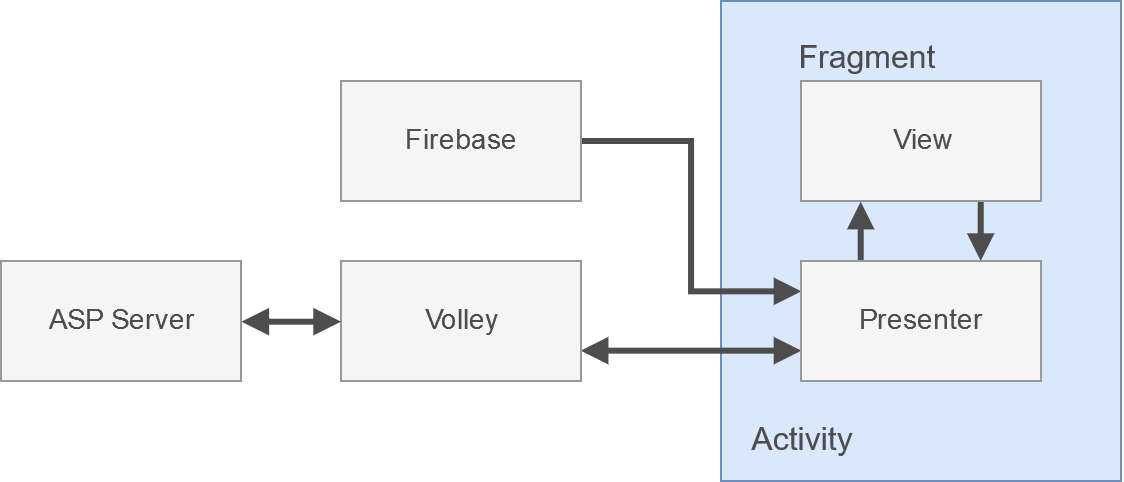
\includegraphics[width=\textwidth]{img/architecture}
\end{figure}

Um die Applikation zu strukturieren wurde hier das Model-View-Presenter Pattern
angewendet. Mit diesem Pattern wird jede Activity in Model-, View- und
Presenter- Komponenten zerlegt. Die Model Komponenten beinhalten die
Zugriffsschicht auf den Event Server mit allen zugehörigen Klassen. In der hier
vorgestellten App wird das Model durch eine \enquote{Network} Singleton Klasse,
welche mit Volley realisiert wurde, und durch entsprechende Entitätsklassen
dargestellt. Ebenfalls werden alle Firebase-Komponenten, die für die
Realisierung des Chat zuständig sind, zum Model gezählt. Man beachte, dass hier
keine klassische Datenbank als Model verwendet wurde. Stattdessen sind alle
Ressourcen nur online zugänglich. Da die hier benötigten Daten design-bedingt
sehr kurzlebig sind, hätte eine lokale Datenbank auf dem Gerät die App
lediglich verkompliziert. Somit stellen der Event- und Firebase-Server das
eigentliche Model dar.

Auf das Model kann nur vom Presenter aus zugegriffen werden. Dieser verwaltet
die eigentlich Logik einer Activity. Dabei ist der Presenter selbst eine
einfache Java Klasse ohne direktes Wissen über das Android System oder die
Datenbank. Events der View werden an den Presenter weitergeleitet und dort
bearbeitet. Der Presenter kann zur Bearbeitung von Events sowohl auf das Model
als auch auf die View Komponenten zugreifen. Diese Komponenten beinhaltet die
Anzeigeschicht und verwaltet die einzelnen GUI-Elemente. In unserer App wird die
View von einer Fragment Klasse implementiert. Direkt kommuniziert die View nur
mit dem Presenter und greift nicht auf das Model zu. In der Praxis gibt es dabei
allerdings einige Ausnahmen.

Um z.B. das Anzeigen von Listen in Android effizient zu realisieren werden
sogenannte Adapter verwendet. Diese greifen meist direkt auf die Datenbank zu
und stellen die erhaltenen Daten direkt in einer ListView da. Damit können diese
Klassen nicht eindeutig den Model oder View Komponenten zugeordnet werden. Daher
implementieren diese meist sowohl die Eigenschaften des Models als auch der
View.

Durch die klare und immer gleichförmige Strukturierung in Model, View und
Presenter, wird das Erstellen von neuen Activities vereinfacht, da somit ein
klarer Arbeitsablauf gegeben ist. Auch das lesen und editieren von fremden Code
wird erleichtert, da von vornherein anhand der Benennung der einzelnen Klassen
klar ist welche Aufgaben diese Komponenten übernehmen.

\newpage

\section{Konzept und Entwurf}
\subsection{Mockups}
Vor dem eigentlichen Implementieren der App wurden Mockups erstellt. Diese
sollten einen ersten Eindruck vom User Interface geben und dienten als
Orientierung während der eigentlichen Implementierung.

An jeder beliebigen Stelle der App hat man Zugriff auf den Navigation Drawer.
Dieser ist ein Menü, welches sich von der linken Seite durch eine Wischgeste
herausziehen lässt. Abbildung ~\ref{drawer} zeigt das Konzept dieses Menüs.

Abbildung ~\ref{singleplayer1} skizziert den Prozess, welchen der Benutzer
vollführen muss, um vom Hauptmenü zum Einzelspieler Modus zu gelangen.

Nach dem das Deck ausgewählt wurde befindet sich der Spieler im eigentlichen
Einzelspieler Modus. Abbildung ~\ref{singleplayer2} skizziert das
Spielgeschehen.

Einstellungen kann der Benutzer in der Settings Activity vornehmen. Allerdings
sind die Möglichkeiten in unserer App sehr beschränkt wie Abbildung
~\ref{settings} zeigt.

Außerdem haben wir Mockups zu den Statistiken erstellt. Hier kann der Benutzer
seine bisherigen Erfolge einsehen. Diese Activity ist auf den Abbildungen
~\ref{stats1} und ~\ref{stats2} zu sehen


\newpage

\section{Implementierung}
\subsection{Übersicht}

\begin{figure}[h!tbp]
  \centering
  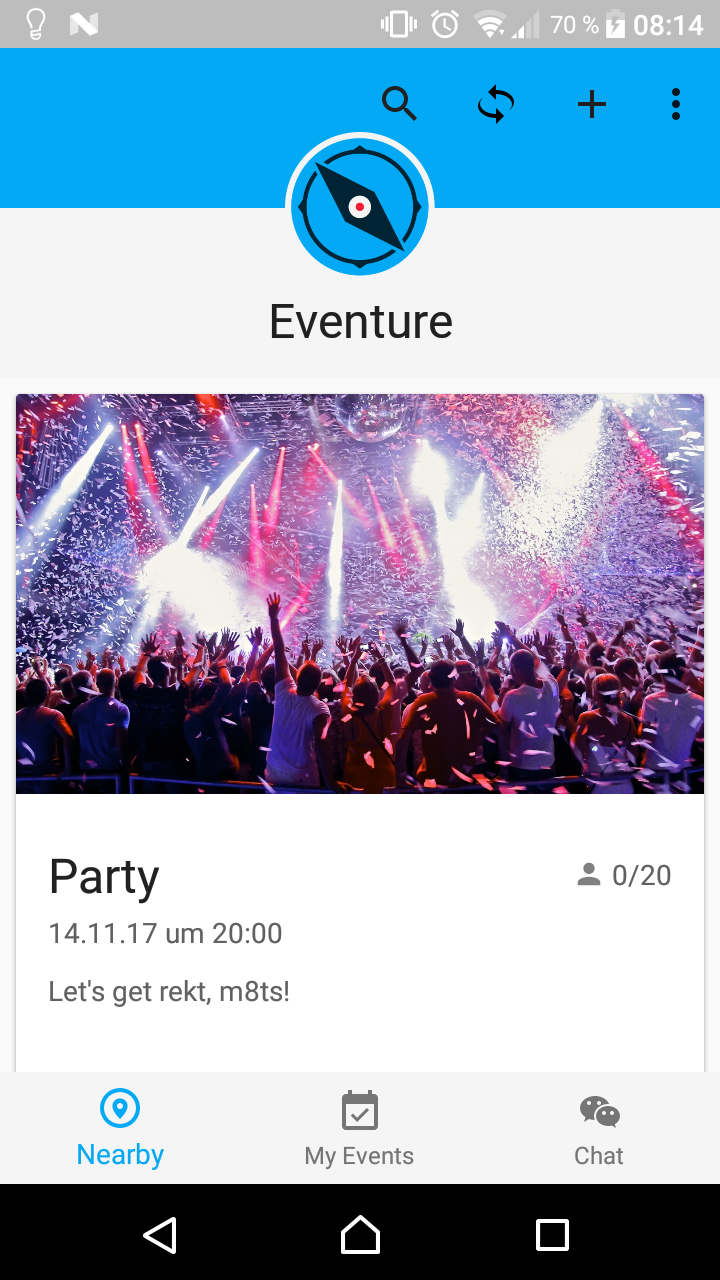
\includegraphics[width=5cm]{img/overview_nearby_1}
  \hspace{1cm}
  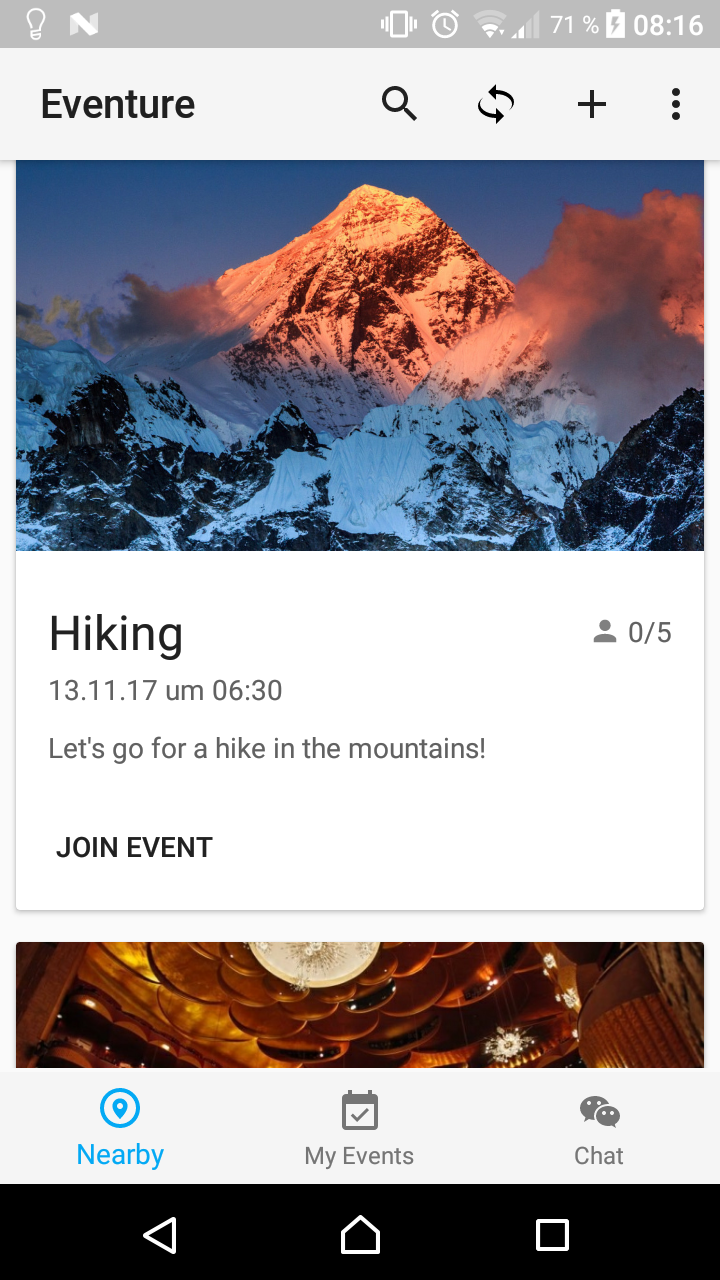
\includegraphics[width=5cm]{img/overview_nearby_2}
  \caption{\enquote{Nearby} Tab der Übersicht}
\end{figure}

Im Startbildschirm erhält der Benutzer eine Übersicht über alle momentan
verfügbaren Events und Chats. In der ActionBar dieser Activity können die
Sucheinstellungen für Events angepasst, neue Events hinzugefügt, und das
Benutzerprofil aufgerufen werden. Durch eine Leiste am unteren Bildschirmrand
kann zwischen in der Nähe befindlichen (\enquote{Nearby}), beigetretenen
Events (\enquote{My Events}) und den zugehörigen Chats (\enquote{Chat})
ausgewählt werden. Dabei werden die Events als eine Liste aus Karten dargestellt
die der Benutzer per Wischgeste durchsuchen kann. Eine Karte zeigt dabei jeweils
das Bild des Events, den Titel, die Beschreibung, den Startzeitpunkt und die
Anzahl der noch freien Plätze. Außerdem werden im unteren Teil der Karte
verschiedene Aktionen als Buttons angezeigt.

\begin{figure}[h!tbp]
  \centering
  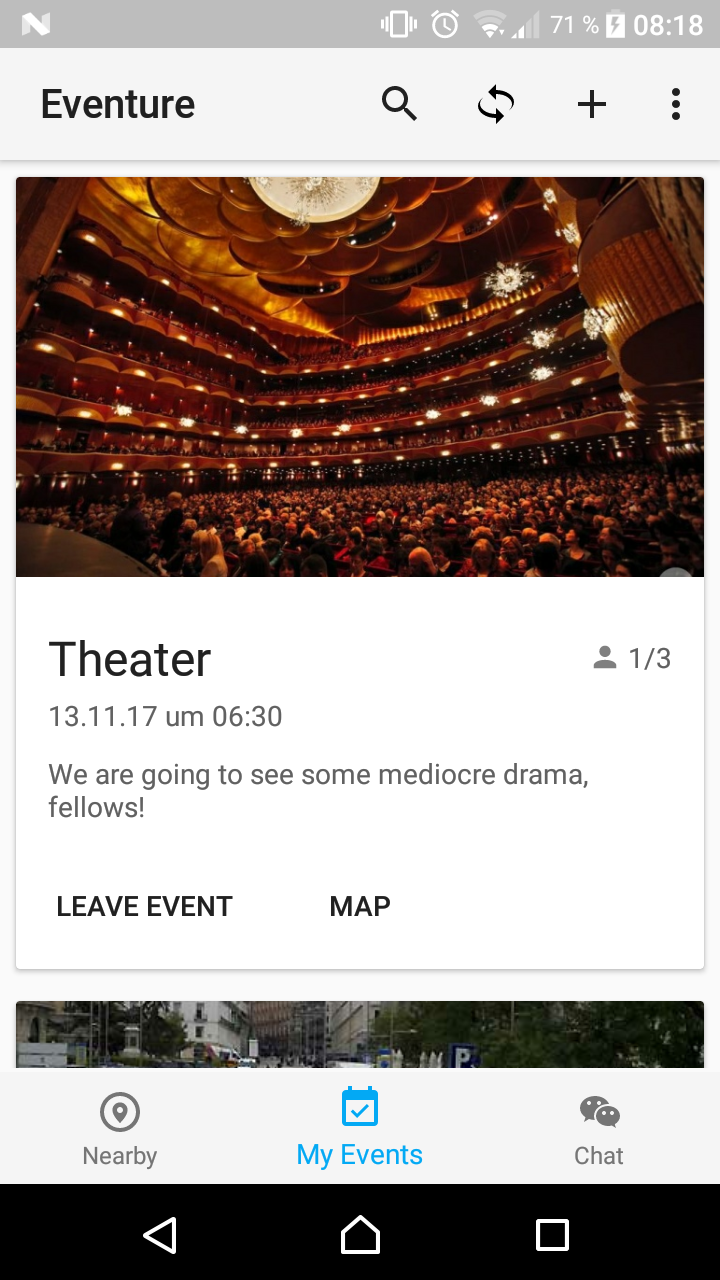
\includegraphics[width=5cm]{img/overview_myevents_1}
  \hspace{1cm}
  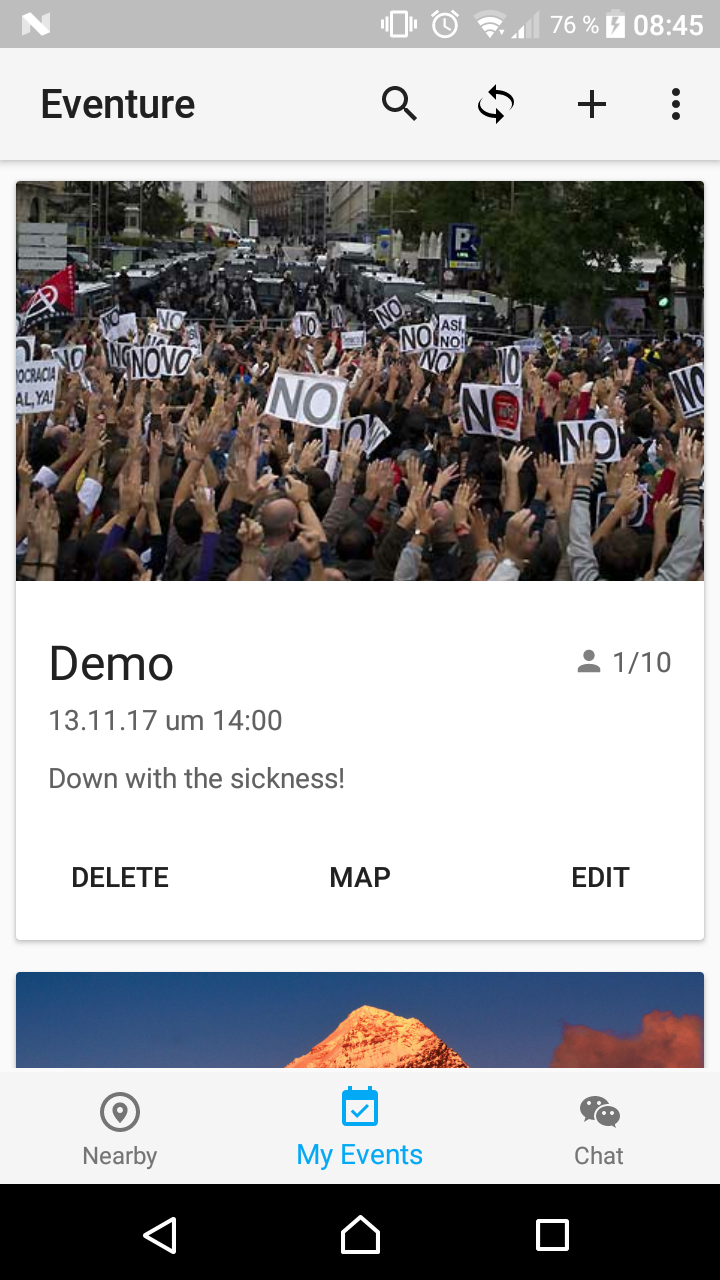
\includegraphics[width=5cm]{img/overview_myevents_2}
  \caption{\enquote{My Events} Tab der Übersicht}
\end{figure}

In der \enquote{Nearby} Liste kann der Benutzer lediglich Events beitreten. Wird
einem Event beigetreten wird eine entsprechende Anfrage an den Event-Server
gesendet. Meldet der Server einen erfolgreichen Beitritt wird daraufhin die
\enquote{Nearby}-Liste aktualisiert, und das Event in die \enquote{My Events}
Liste eingefügt. Events in dieser Liste stellen dem Benutzer entweder die
Aktionen \enquote{Map} und \enquote{Leave} \emph{oder} \enquote{Delete},
\enquote{Map} und \enquote{Edit} bereit. Dabei werden Letztere nur für
diejenigen Events angezeigt, welche der Benutzer selbst erstellt hat. Ist der
Benutzer einem Event begetreten, hat dieses aber nicht selbst erstellt so wird
statt \enquote{Delete} der Button \enquote{Leave} angezeigt. Tippt der Benutzer
auf den \enquote{Delete} Button wird eine Anfrage an den Event-Server und an die
Firebase-Datenbank gesendet, die auf dem Event-Server das Event und in Firebase
den zugehörigen Chat aus der Datenbank löscht. Wird der \enquote{Leave} Button
betätigt wird nur der Benutzer aus dem Event entfernt. Das Event selbst bleibt
aber bestehen und ist wieder in der \enquote{Nearby}-Liste auffindbar. Ein Event
hat somit immer mindestens den erstellenden Benutzer als Teilnehmer. Der
außerdem verfügbare \enquote{Map} Button öffnet über einen speziell formatierten
\emph{Intent} die Google Maps App und zeigt den Ort des Events an. So können
Benutzer schnell zum Ort des Events navigieren. Über den \enquote{Edit} Button
kann der erstellende Benutzer nachträglich die Details eines Events bearbeiten.

Alle diese Events werden asynchron direkt vom Event-Server geladen und nicht
zwischengespeichert. Somit wird garantiert, dass immer nur aktuelle Events
angezeigt werden. Als Übertragungsformat wird hier JSON verwendet. Ein
JSON-Objekt repräsentiert dabei ein komplettes Event, wobei das zugehörige Bild
über eine separate URL vom Server geladen wird. Auch die Liste an verfügbaren
Chats wird asynchron geladen und nicht zwischengespeichert. Die Daten werden
dabei allerdings von Firebase geladen, wobei das bereitgestellte Firebase-API
verwendet wurde. Dieses liefert die angeforderten Objekte als
\emph{DataSnapshot} Instanzen zurück, die mittels Reflection in Objekte einer
passenden Java Klasse umgewandelt werden können. Außerdem wird die App über die
Firebase-API über Änderungen an der Chat Liste benachrichtigt. Anhand dieser
Änderungen wird die dargestellte Liste aktualisiert, womit diese immer aktuell
gehalten wird.

Die verschiedenen Listen des Startbildschirms werden über drei verschiedene
Fragments realisiert. Dabei werden alle drei Fragments beim Erstellen der
zughörigen Activity instanziiert und während des Bestehens der Activity
permanent im Speicher gehalten. Die Activity selbst beinhaltet neben der unteren
Navigationsleiste lediglich ein Frame Layout, in welches die Fragments
platzierte werden können. Wird eine Liste ausgewählt wird einfach das zughörige
Fragment in das Frame Layout geladen.

\subsection{Kartenansicht}

\begin{figure}[h!tbp]
  \centering
  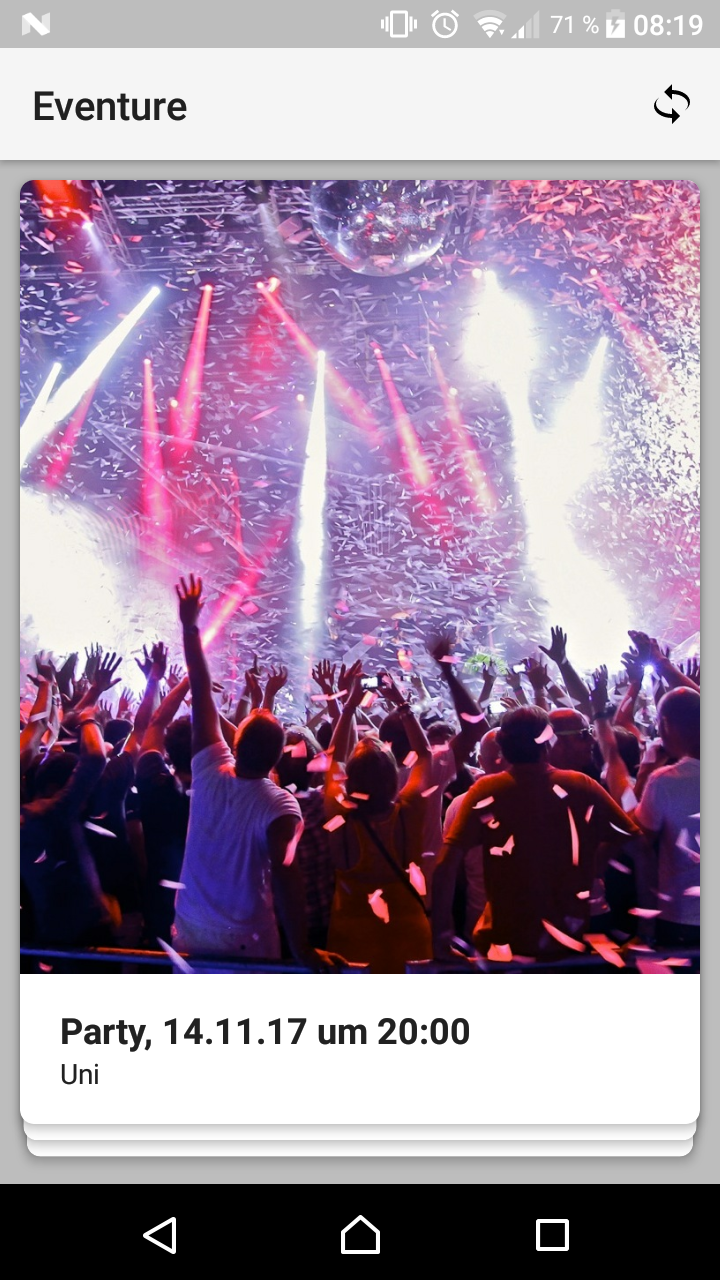
\includegraphics[width=5cm]{img/cardview}
  \caption{Kartenansicht der verfügbaren Events}
\end{figure}

In dieser Ansicht werden alle Events angezeigt die auch in der \enquote{Nearby}
Liste in der Übersicht angezeigt werden. Dabei werden die Events hier allerdings
nicht als eine kontinuierliche Liste präsentiert sondern als ein simulierter
Kartenstapel. Jede Karte beinhaltet nur minimale Information und bietet
hauptsächlich Platz für das Bild des Events. So soll eine spontane Entscheidung
über das Gefallen oder Nicht-Gefallen des Events unterstützt werden.

\begin{figure}[h!tbp]
  \centering
  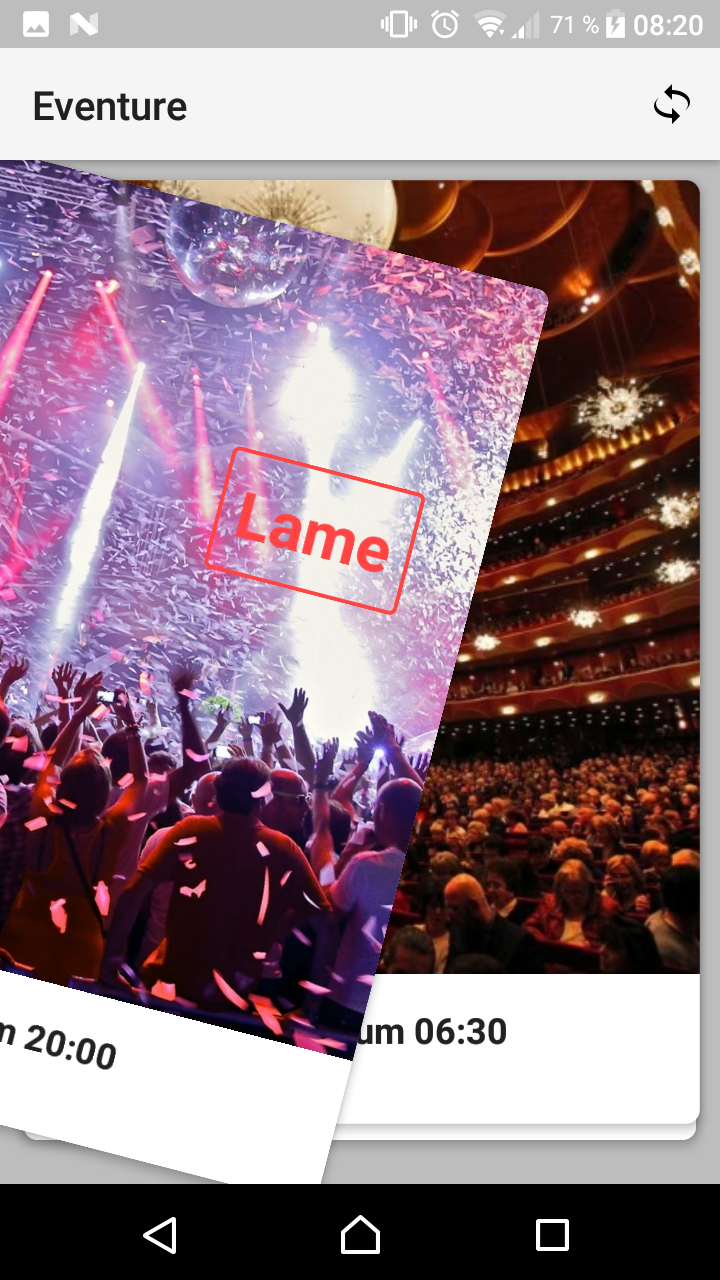
\includegraphics[width=5cm]{img/cardview_lame}
  \hspace{1cm}
  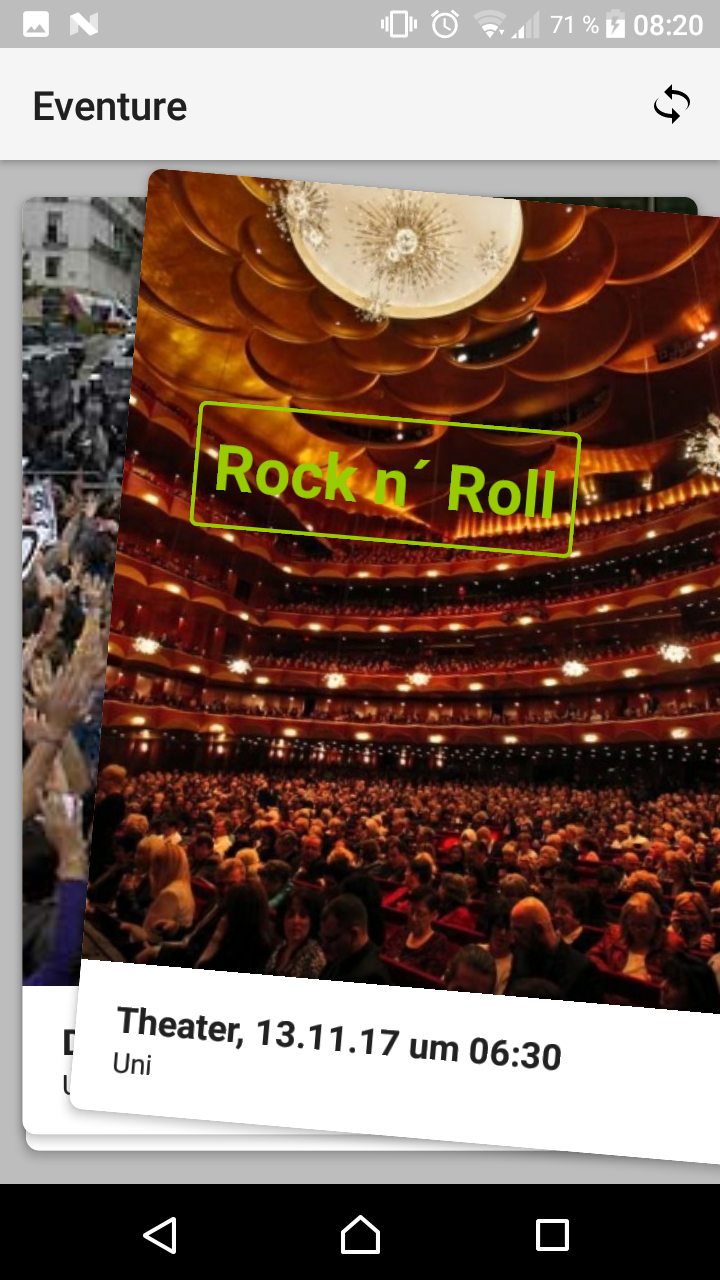
\includegraphics[width=5cm]{img/cardview_rocknroll}
  \caption{Event wird abgelehnt oder dem Event wird beigetreten}
\end{figure}

Wird die Karten nach rechts geschoben tritt der Benutzer dem Event bei. Wird die
Karte dagegen nach links geschoben tritt der Benutzer dem Event nicht bei und
die Karte wird wieder in den virtuellen Kartenstapel eingeordnet. Dieser Stapel
wird hier durch die \emph{PlaceHolderView} realisiert. Die anzuzeigenden Events
werden dabei ebenfalls direkt vom Event-Server und nicht aus einer lokalen
Datenbank geladen.

\subsection{Event Erstellung}

\begin{figure}[h!tbp]
  \centering
  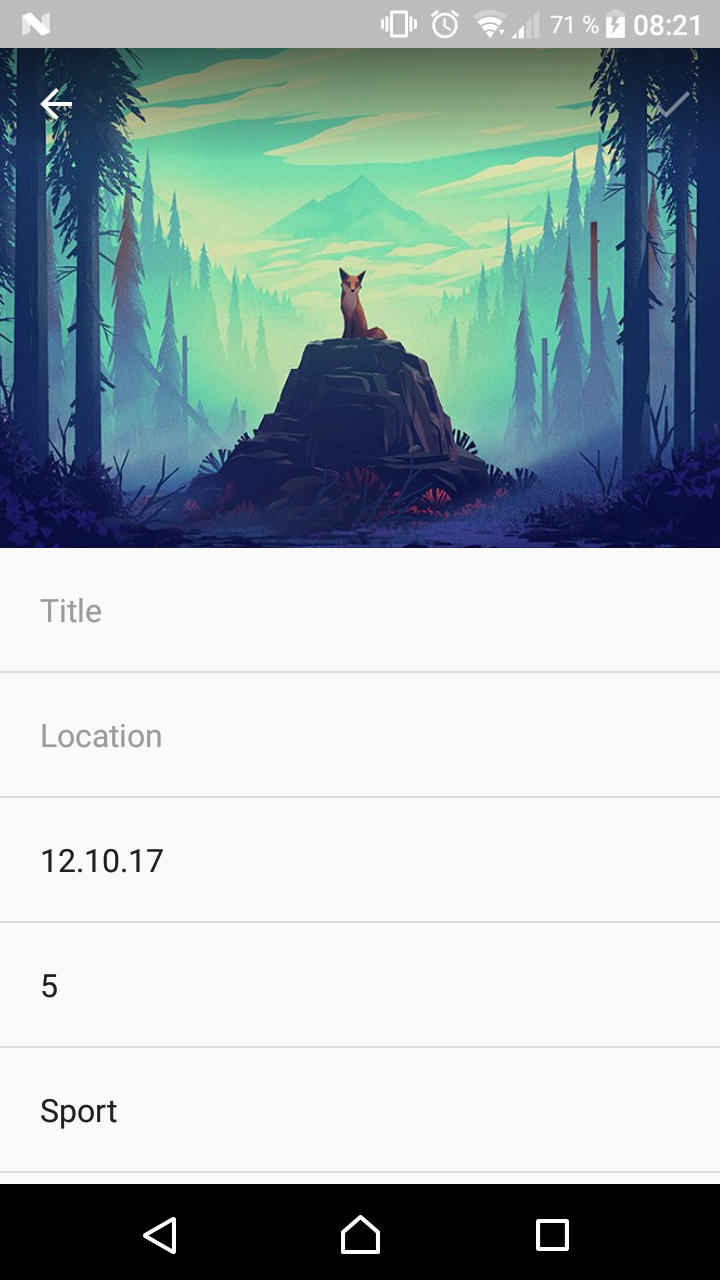
\includegraphics[width=5cm]{img/addevent_1}
  \caption{View zur Event Erstellung}
\end{figure}

In dieser Activity kann ein Benutzer ein Event anlegen oder ein bereits
bestehendes Event bearbeiten. Die dafür nötige Eingabemaske wurde dabei so
einfach und klar wie möglich strukturiert. Den Großteil der vorhandenen Fläche
nimmt eine ImageView ein, in welcher das zugehörige Bild des Events angezeigt
wird. Um die Fläche für dieses Bild zusätzlich zu maximieren wurde hier die
ActionBar der Activity transparent dargestellt. Damit der weiße
\enquote{Zurück}-Button der Activity immer noch sichtbar bleibt wird die
ActionBar aber nicht komplett transparent sondern mit einem leichten Farbverlauf
gezeichnet. Dieser Farbverlauf ist über dem Bild der ImageView kaum sichtbar,
aber erhöht dennoch merklich die Sichtbarkeit des \enquote{Zurück}-Buttons.
Klick der Benutzer auf das Bild kann er ein beliebiges auf dem Gerät vorhandenes
Bild auswählen, das dann in der ImageView angezeigt wird. Dabei wird das Bild
asynchron im Hintergrund, dass heißt abseits des Haupt-Threads geladen.

\begin{figure}[h!tbp]
  \centering
  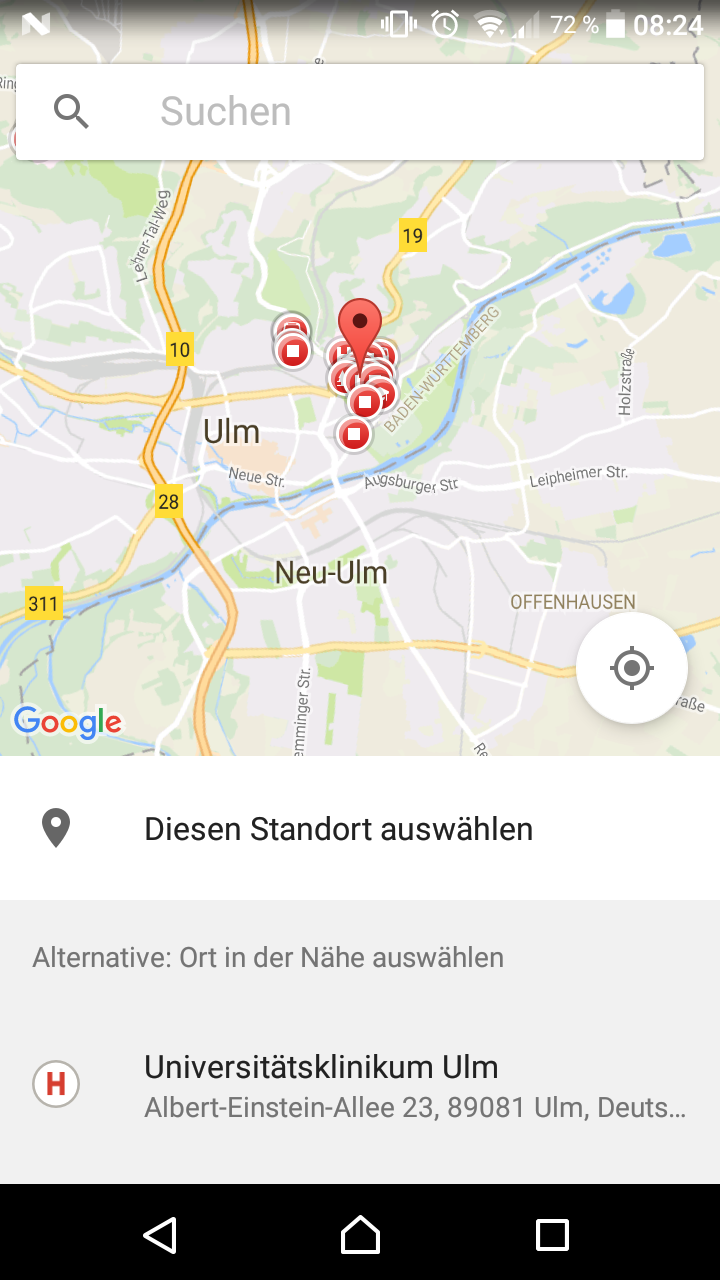
\includegraphics[width=5cm]{img/addevent_places}
  \hspace{1cm}
  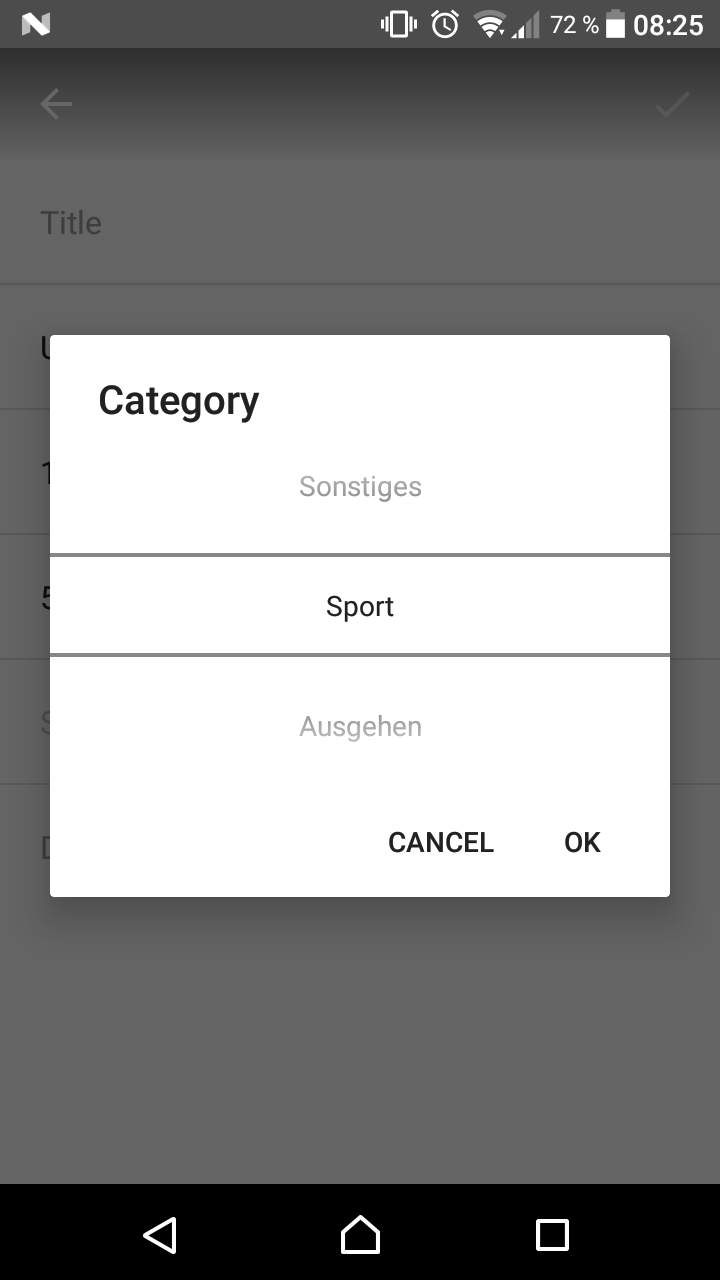
\includegraphics[width=5cm]{img/addevent_category}
  \caption{Picker zur Orts- und Kategorieauswahl}
\end{figure}

In den dann folgenden Textfeldern können die weiteren Parameter des Events
konfiguriert werden. Dabei wurde das Design der Textfelder so angepasst, dass
diese die gesamte Bildschirmbreite verwendet. Damit wurde auch auch die
klickbare Fläche der Textfelder vergrößert, sodass das Auswählen eines einzelnen
Textfelds einfacher möglich ist. Obwohl als Anzeige Textfelder verwendet werden
sind diese nur bedingt für die Auswahl einiger Informationen geeigent. Klickt
der Benutzer z.B. auf das \enquote{Location} Textfeld wird über das Google
Places API eine Place Picker Activity gestartet die eine benutzerfreundliche
Auswahl eines Ortes ermöglicht. Der ausgewählte Ort wird intern gespeichert und
eine textuelle Repräsentation des Ortes im zugehörigen Textfeld angezeigt. Um
die Startzeit auszuwählen wurde ein Time-Picker-Dialog erstellt, der geöffnet
wird, wenn der Benutzer auf das \enquote{Start} Textfeld tippt. So kann eine
Startzeit benutzerfreundlich eingegeben werden. Auch werden so
Formatierungsfehler vermieden, die bei der Eingabe von Daten in ein Textfeld
auftreten können. Ebenfalls wurden Picker-Dialoge für die Felder
\enquote{Max participants} und \enquote{Category} erstellt.

\begin{figure}[h!tbp]
  \centering
  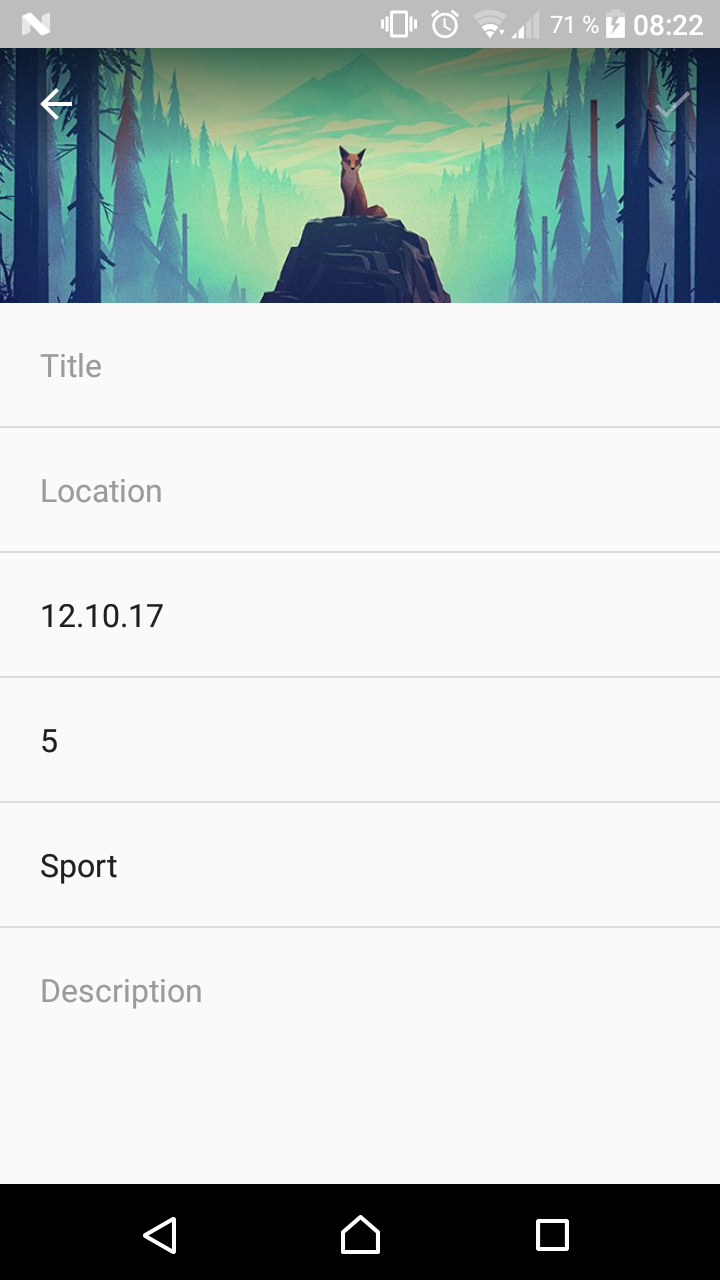
\includegraphics[width=5cm]{img/addevent_2}
  \hspace{1cm}
  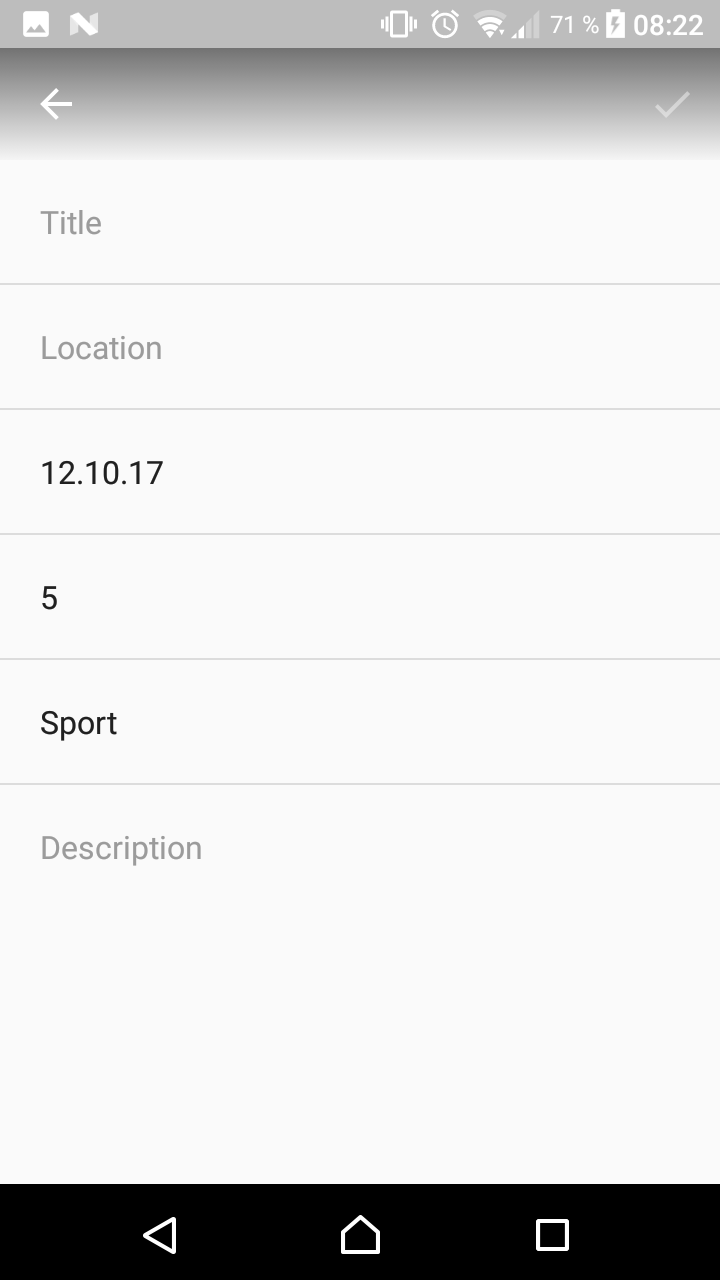
\includegraphics[width=5cm]{img/addevent_3}
  \caption{Scroll-Verhalten mit \emph{NestedScrollView} und \emph{AppBarLayout}}
\end{figure}

Aufgrund der relative großen Darstellung des Bilds können nicht alle benötigten
Felder auf einer Bildschirmlänge dargestellt werden. Daher musste die
Parameterliste scrollbar implementiert werden. Um von jeder Scroll-Position die
Activity wieder verlassen zu können muss der \enquote{Zurück}-Button, dass heißt
die ActionBar der Activity, immer zugänglich bleiben. Allerdings wurde diese
transparent gezeichnet und ist somit auf den Textfeldern schlecht lesbar. Daher
wurde hier eine \emph{NestedScrollView} in Kombination mit einem
\emph{AppBarLayout} verwendet. Wird auf der Parameterliste gescrollt schiebt
sich diese über das Bild des Events und der Hintergrund der AppBar wird so
transformiert, dass dieser nun nicht mehr transparent ist. Somit kann nun der
\enquote{Zurück}-Button immer angezeigt und die Parameterliste gescrollt werden.

\subsection{Server}

\section{Anforderungsabgleich}

Im Folgenden werden die gegebenen Anforderungen mit der tatsächlichen
Implementierung verglichen. Es wird festgestellt ob eine Anforderung ganz,
teilweise oder gar nicht erfüllt wurde.

\subsection{Funktionale Anforderungen}

\textbf{FA1 Hauptmenü - erfüllt} \newline
Das Hauptmenü wurde wie in der Anforderung beschrieben implementiert.

\ \newline
\textbf{FA2 Spielmodi - erfüllt} \newline
Alle Spielmodi wurden wie gefordert implementiert und können vor jedem Spiel
ausgewählt werden.

\ \newline
\textbf{FA3 Computergegner - erfüllt} \newline
Für den Einzelspielermodus wurde ein Computergegner implementiert, der ein
faires Spielerlebnis bietet. Diese \enquote{KI} kann je nach Schwierigkeitsgrad
unterschiedlich gut abschätzen welches Attribut einer Karte die höchsten
Gewinnchancen hat und imitiert so das Verhalten eines menschlichen Spielers.

\ \newline
\textbf{FA4 Schwierigkeitsgrad - erfüllt} \newline
Die geforderten Schwierigkeitsgrade wurden implementiert und können vor dem
Beginn eines neuen Spiels ausgewählt werden. Die Wahl des Schwierigkeitsgrads
beeinflusst das Verhalten der KI.

\ \newline
\textbf{FA5 Spiel fortsetzen - erfüllt} \newline
Nach jedem Spielzug wird der komplette Zustand des Spiels in die interne
Datenbank geschrieben und damit persistent gespeichert.

\ \newline
\textbf{FA6 Galerie - erfüllt} \newline
Die Galerie wurde wie in \enquote{Implementierungsdetails} beschreiben
implementiert.

\ \newline
\textbf{FA7 Deck Download - erfüllt} \newline
Der Deckdownload wurde wie in \enquote{Implementierungsdetails} beschreiben in
die Galerie integriert.

\ \newline
\textbf{FA8 Statistiken - erfüllt} \newline
Die Statistiken wurden implementiert und werden graphisch aufbereitet in einer
speziellen Ansicht dargestellt.

\ \newline
\textbf{FA9 Rangliste - erfüllt} \newline
Die beschriebene Rangliste wurde implementiert. Der Spieler wird mit dem Namen
der zu Beginn eines Spiels eingegeben wurde, automatisch mit seiner erreichten
Punktezahl in die Rangliste aufgenommen

\ \newline
\textbf{FA10 Achievements - teilweise erfüllt} \newline
Es wurde eine Oberfläche zur Anzeige der Achievements implementiert. Ein
fertiges Achievementsystem ist allerdings nicht in der App vorhanden.

\ \newline
\textbf{FA11 Quartetteditor - nicht erfüllt} \newline
Der Quartetteditor wurde zugunsten des Multiplayers nicht realisiert.

\ \newline
\textbf{FA12 Levelsystem - nicht erfüllt} \newline
Das Levelsystem wurde zugunsten des Multiplayers nicht realisiert

\ \newline
\textbf{FA13 Multiplayer - erfüllt} \newline
Der Multiplayer wurde mit Hilfe der Google Play Services implementiert und
erlaubt es zwei Benutzer der App über das Internet gegeneinander anzutreten.

\subsection{Nicht Funktionale Anforderungen}

\textbf{NFA1 Robustheit - teilweise} \newline
Der Multiplayer weist aufgrund der Komplexität und fehlender Entwicklungszeit
noch einige Stabilitätsprobleme auf. Ansonsten konnten während der Entwicklung
keine Fehler festgestellt werden, welche die Robustheit der App beinträchtigen.

\ \newline
\textbf{NFA2 Erweiterbarkeit - erfüllt} \newline
Durch die Verwendung des Model-View-Presenter Patterns ist eine einfache
Erweiterbarkeit gegeben.

\ \newline
\textbf{NFA3 Responsiveness - erfüllt} \newline
Durch den permanenten Einsatz von asynchronen Programmiertechniken wurde
sichergestellt, dass die Applikation immer entsprechend schnell reagiert.

\ \newline
\textbf{NFA4 Usability - erfüllt} \newline
Um die Usability sicher zu stellen wurden die Google User Interface Guidelines
als Referenz für die Gestaltung der Oberflächen verwendet.

\section{Zusammenfassung und Ausblick}

In dieser Dokumentation wurde die Planung der Entwicklung einer Android Quartett
App und die tatsächlich Implementierung dieser vorgestellt. Da die allermeisten
der funktionale und nicht funktionalen Anforderungen erfüllt wurden, kann das
Projekt als erfolgreich bewertet werden. Darüberhinaus konnten wir zahlreiche
Einblicke in die Entwicklung von Android Applikationen erhalten. Wir sind nun
mit den wichtigsten Konzepten der Plattform vertraut, sodass die Entwicklung
weiterer Apps deutlich einfacher zu bewerkstelligen sein wird. Außerdem konnten
wir zusätzliche Erkenntnisse in der Verwendung von Design Patterns und des
Versionskontrollsystems git sammeln.

\ \newline
Aufgrund der gewonnen Erkenntnisse und des allgemein guten Projektverlaufs werden
wir auch weiter Apps mit Android und unter zu Hilfenahme der hier verwendeten
Werkzeuge und Strategien entwickeln.

\end{document}
